% Options for packages loaded elsewhere
\PassOptionsToPackage{unicode}{hyperref}
\PassOptionsToPackage{hyphens}{url}
\PassOptionsToPackage{dvipsnames,svgnames*,x11names*}{xcolor}
%
\documentclass[
  ignorenonframetext,
]{beamer}
\usepackage{pgfpages}
\setbeamertemplate{caption}[numbered]
\setbeamertemplate{caption label separator}{: }
\setbeamercolor{caption name}{fg=normal text.fg}
\beamertemplatenavigationsymbolsempty
% Prevent slide breaks in the middle of a paragraph
\widowpenalties 1 10000
\raggedbottom
\setbeamertemplate{part page}{
  \centering
  \begin{beamercolorbox}[sep=16pt,center]{part title}
    \usebeamerfont{part title}\insertpart\par
  \end{beamercolorbox}
}
\setbeamertemplate{section page}{
  \centering
  \begin{beamercolorbox}[sep=12pt,center]{part title}
    \usebeamerfont{section title}\insertsection\par
  \end{beamercolorbox}
}
\setbeamertemplate{subsection page}{
  \centering
  \begin{beamercolorbox}[sep=8pt,center]{part title}
    \usebeamerfont{subsection title}\insertsubsection\par
  \end{beamercolorbox}
}
\AtBeginPart{
  \frame{\partpage}
}
\AtBeginSection{
  \ifbibliography
  \else
    \frame{\sectionpage}
  \fi
}
\AtBeginSubsection{
  \frame{\subsectionpage}
}
\usepackage{amsmath,amssymb}
\usepackage{lmodern}
\usepackage{ifxetex,ifluatex}
\ifnum 0\ifxetex 1\fi\ifluatex 1\fi=0 % if pdftex
  \usepackage[T1]{fontenc}
  \usepackage[utf8]{inputenc}
  \usepackage{textcomp} % provide euro and other symbols
\else % if luatex or xetex
  \usepackage{unicode-math}
  \defaultfontfeatures{Scale=MatchLowercase}
  \defaultfontfeatures[\rmfamily]{Ligatures=TeX,Scale=1}
\fi
% Use upquote if available, for straight quotes in verbatim environments
\IfFileExists{upquote.sty}{\usepackage{upquote}}{}
\IfFileExists{microtype.sty}{% use microtype if available
  \usepackage[]{microtype}
  \UseMicrotypeSet[protrusion]{basicmath} % disable protrusion for tt fonts
}{}
\makeatletter
\@ifundefined{KOMAClassName}{% if non-KOMA class
  \IfFileExists{parskip.sty}{%
    \usepackage{parskip}
  }{% else
    \setlength{\parindent}{0pt}
    \setlength{\parskip}{6pt plus 2pt minus 1pt}}
}{% if KOMA class
  \KOMAoptions{parskip=half}}
\makeatother
\usepackage{xcolor}
\IfFileExists{xurl.sty}{\usepackage{xurl}}{} % add URL line breaks if available
\IfFileExists{bookmark.sty}{\usepackage{bookmark}}{\usepackage{hyperref}}
\hypersetup{
  pdftitle={Chapter 7},
  colorlinks=true,
  linkcolor=Maroon,
  filecolor=Maroon,
  citecolor=Blue,
  urlcolor=blue,
  pdfcreator={LaTeX via pandoc}}
\urlstyle{same} % disable monospaced font for URLs
\newif\ifbibliography
\usepackage{graphicx}
\makeatletter
\def\maxwidth{\ifdim\Gin@nat@width>\linewidth\linewidth\else\Gin@nat@width\fi}
\def\maxheight{\ifdim\Gin@nat@height>\textheight\textheight\else\Gin@nat@height\fi}
\makeatother
% Scale images if necessary, so that they will not overflow the page
% margins by default, and it is still possible to overwrite the defaults
% using explicit options in \includegraphics[width, height, ...]{}
\setkeys{Gin}{width=\maxwidth,height=\maxheight,keepaspectratio}
% Set default figure placement to htbp
\makeatletter
\def\fps@figure{htbp}
\makeatother
\setlength{\emergencystretch}{3em} % prevent overfull lines
\providecommand{\tightlist}{%
  \setlength{\itemsep}{0pt}\setlength{\parskip}{0pt}}
\setcounter{secnumdepth}{-\maxdimen} % remove section numbering
\usepackage{multirow} \usepackage{graphicx} \graphicspath{{images/}} \usepackage{subfigure} \usepackage{multicol} \usepackage[utf8]{inputenc} \usepackage[english]{babel} \usepackage{bm} \usepackage{amsmath} \usepackage{tikz} \usepackage{mathtools} \usepackage{textcomp} \usepackage{fdsymbol} \usepackage{siunitx} \usepackage{xcolor,pifont} \usepackage{hyperref} \usepackage{mathtools}
\ifluatex
  \usepackage{selnolig}  % disable illegal ligatures
\fi

\title{Chapter 7}
\subtitle{Inference for numerical data\footnote<.->{These notes use
  content from OpenIntro Statistics Slides by Mine Cetinkaya-Rundel.}}
\author{Department of Mathematics \& Statistics\\
North Carolina A\&T State University}
\date{}

\begin{document}
\frame{\titlepage}

\hypertarget{computing-the-power-for-a-2-sample-test}{%
\section{Computing the power for a 2-sample
test}\label{computing-the-power-for-a-2-sample-test}}

\begin{frame}{}
\protect\hypertarget{section}{}
\begin{center}
\begin{tabular}{l l | c c}
\multicolumn{2}{c}{} & \multicolumn{2}{c}{\textbf{Decision}} \\
& & fail to reject $H_0$ &  reject $H_0$ \\
  \cline{2-4}
& $H_0$ true & \onslide<4->{\textcolor{blue}{$1 - \alpha$}} & \onslide<2->{\textcolor{orange}{Type 1 Error, $\alpha$}} \\
\raisebox{1.5ex}{\textbf{Truth}} & $H_A$ true &  \onslide<3->{\textcolor{orange}{Type 2 Error, $\beta$}} & \onslide<5->{\textcolor{blue}{Power, $1 - \beta$}} \\
  \cline{2-4}
\end{tabular}
\end{center}

\pause

\begin{itemize}
\item Type 1 error is rejecting $H_0$ when you shouldn't have, and the probability of doing so is $\alpha$ (significance level)

\pause 

\item Type 2 error is failing to reject $H_0$ when you should have, and the probability of doing so is $\beta$ (a little more complicated to calculate)

\pause 

\item \textbf{Power} of a test is the probability of correctly rejecting $H_0$, and the probability of doing so is $1 - \beta$

\pause 

\item In hypothesis testing, we want to keep $\alpha$ and $\beta$ low, but there are inherent trade-offs.

\end{itemize}
\end{frame}

\begin{frame}{Type 2 error rate}
\protect\hypertarget{type-2-error-rate}{}
If the alternative hypothesis is actually true, what is the chance that
we make a Type 2 Error, i.e.~we fail to reject the null hypothesis even
when we should reject it?

\begin{itemize}
\item
  The answer is not obvious.
\item
  If the true population average is very close to the null hypothesis
  value, it will be difficult to detect a difference (and reject
  \(H_0\)).
\item
  If the true population average is very different from the null
  hypothesis value, it will be easier to detect a difference.
\item
  Clearly, \(\beta\) depends on the \textbf{effect size} (\(\delta\)).
\end{itemize}
\end{frame}

\begin{frame}{Example - Blood Pressure (BP), hypotheses}
\protect\hypertarget{example---blood-pressure-bp-hypotheses}{}
\alert{Suppose a pharmaceutical company has developed a new drug for lowering blood pressure, and they are preparing a clinical trial to test the drug's effectiveness. They recruit people who are taking a particular standard blood pressure medication, and half of the subjects are given the new drug (treatment) and the other half continue to take their current medication through generic-looking pills to ensure blinding (control). What are the hypotheses for a two-sided hypothesis test in this context?}

\pause

\begin{align*}
H_0&: \mu_{treatment} - \mu_{control} = 0 \\
H_A&: \mu_{treatment} - \mu_{control} \ne 0  
\end{align*}
\end{frame}

\begin{frame}{Example - BP, standard error}
\protect\hypertarget{example---bp-standard-error}{}
\alert{Suppose researchers would like to run the clinical trial on patients with systolic blood pressures between 140 and 180 mmHg. Suppose previously published studies suggest that the standard deviation of the patients' blood pressures will be about 12 mmHg and the distribution of patient blood pressures will be approximately symmetric. If we had 100 patients per group, what would be the approximate standard error for difference in sample means of the treatment and control groups?}

\pause

\centering{$SE = \sqrt{\frac{12^2}{100} + \frac{12^2}{100}} = 1.70$}
\end{frame}

\begin{frame}{Example - BP, minimum effect size required to reject
\(H_0\)}
\protect\hypertarget{example---bp-minimum-effect-size-required-to-reject-h_0}{}
\alert{For what values of the difference between the observed averages of blood pressure in treatment and control groups (effect size) would we reject the null hypothesis at the 5\% significance level?}

\pause

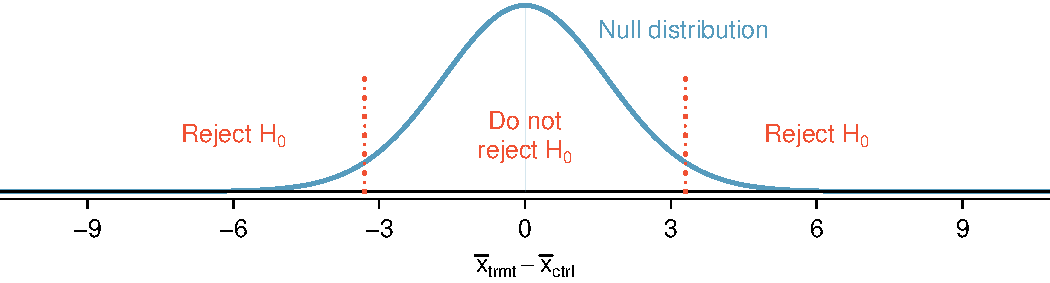
\includegraphics[width=\textwidth,height=0.5\textheight]{power_null_B_0_1-7_with_rejection_region.pdf}

\pause

The difference should be at least

\centering{$1.96 \times 1.70 = 3.332.$}

\raggedright or at most

\centering{$-1.96 \times 1.70 = -3.332.$}
\end{frame}

\begin{frame}{Example - BP, power}
\protect\hypertarget{example---bp-power}{}
\alert{Suppose that the company researchers care about finding any effect on blood pressure that is 3 mmHg or larger vs the standard medication. What is the power of the test that can detect this effect?}

\pause

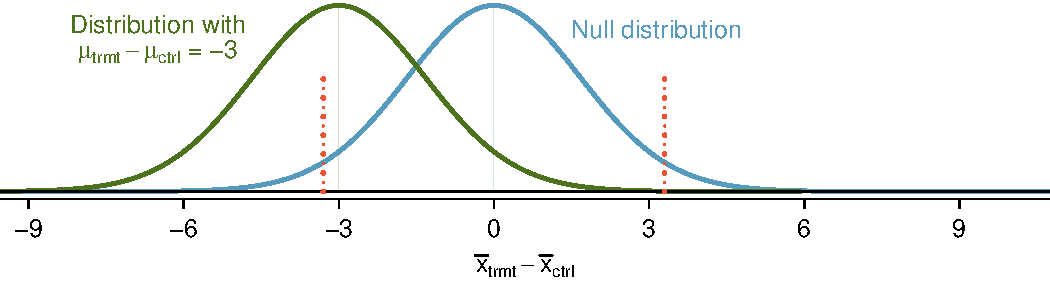
\includegraphics[width=\textwidth,height=0.5\textheight]{power_null_C_0_1-7_with_alt_at_3.pdf}

\pause

\centering{$Z = \frac{-3.332-(-3)}{1.70} = 0.20$}

\pause

\centering{$P(Z < -0.20) = 0.4207$}
\end{frame}

\begin{frame}{Example - BP, required sample size for 80\% power}
\protect\hypertarget{example---bp-required-sample-size-for-80-power}{}
\alert{What sample size will lead to a power of 80\% for this test?}

\pause

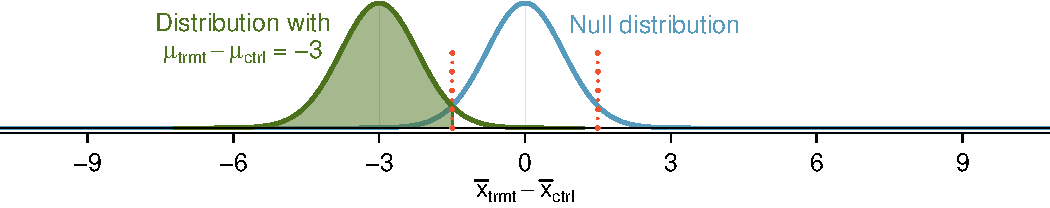
\includegraphics[width=\textwidth,height=0.5\textheight]{power_null_0_0-76_with_alt_at_3_and_shaded.pdf}

\pause

\centering{$SE = \frac{3}{2.8} = 1.07142$}

\pause

\centering{$1.07142 = \sqrt{\frac{12^2}{n} + \frac{12^2}{n}}$}

\pause

\centering{$n = 250.88 \rightarrow n \geq 251$}
\end{frame}

\begin{frame}{Recap}
\protect\hypertarget{recap}{}
\begin{itemize}
\item
  Calculate required sample size for a desired level of power.
\item
  Calculate power for a range of sample sizes, then choose the sample
  size that yields the target power (usually 80\% or 90\%).
\end{itemize}

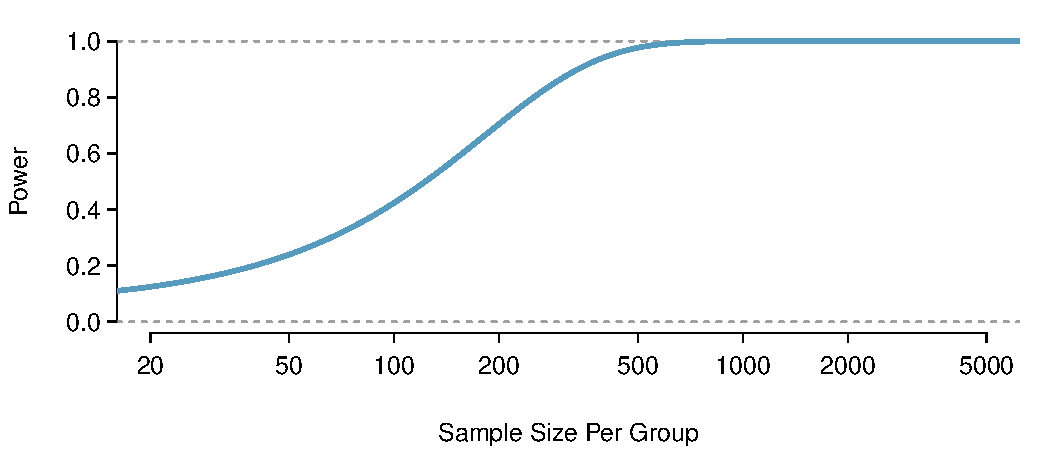
\includegraphics[width=\textwidth,height=0.7\textheight]{power_curve_neg-3.pdf}
\end{frame}

\begin{frame}{Achieving desired power}
\protect\hypertarget{achieving-desired-power}{}
There are several ways to increase power (and hence decrease type 2
error rate):

\pause

\begin{enumerate}

\item Increase the sample size.

\pause

\item Decrease the standard deviation of the sample, which essentially has the same effect as increasing the sample size (it will decrease the standard error). With a smaller $s$ we have a better chance of distinguishing the null value from the observed point estimate. This is difficult to ensure but cautious measurement process and limiting the population so that it is more homogeneous may help.

\pause

\item Increase $\alpha$, which will make it more likely to reject $H_0$ (but note that this has the side effect of increasing the Type 1 error rate).

\pause

\item Consider a larger effect size. If the true mean of the population is in the alternative hypothesis but close to the null value, it will be harder to detect a difference.

\end{enumerate}
\end{frame}

\end{document}
